\chapter{Projekt systemu Team Challenge}

W niniejszym rozdziale ...

\section{Grupa docelowa}

Grupa docelowa, wiek itp.

\section{Wymagania funkcjonalne}

Wymagania funkcjonalne...

\subsubsection{Konta użytkowników}


\begin{table}[H]
\centering\small
\caption{Wymagania funkcjonalne - konta użytkowników}
\label{tab:szablon}
\begin{tabularx}{\linewidth}{|p{.2\linewidth}|X|}\hline
Nr. ident. & Opis \\ \hline\hline

FR-USR-01 & Gość na stronie może założyć konto w systemie podając: adres email, hasło, imię, nazwisko oraz datę urodzenia. \\ \hline
FR-USR-02 & Użytkownik systemu może modyfikować wprowadzone przez siebie dane.  \\ \hline
FR-USR-03 & Użytkownik systemu może usunąć swoje konto.  \\ \hline

\end{tabularx}
\end{table}

\subsubsection{Profile zawodników}


\begin{table}[H]
\centering\small
\caption{Wymagania funkcjonalne - profile zawodników}
\label{tab:szablon}
\begin{tabularx}{\linewidth}{|p{.2\linewidth}|X|}\hline
Nr. ident. & Opis \\ \hline\hline

FR-PLR-01 & Użytkownik może utworzyć profil zawodnika. Użytkownik dokonuje wyboru regionu, wprowadza swój wzrost, deklaruje poziom umiejętności oraz częstość gry.   \\ \hline
FR-PLR-02 & Użytkownik może zarządzać swoim profilem zawodnika.  \\ \hline

\end{tabularx}
\end{table}

\subsubsection{Tworzenie drużyn i rekrutacja}

\subsubsection{Zarządzanie obiektami sportowymi}

\subsubsection{Poszukiwanie rywali}

\subsubsection{Organizacja spotkań}

\begin{table}[H]
\centering\small
\caption{Wymagania funkcjonalne - negocjacje}
\label{tab:szablon}
\begin{tabularx}{\linewidth}{|p{.2\linewidth}|X|}\hline
Nr. ident. & Opis \\ \hline\hline

FR-NEG-01 & Kapitan drużyny może rzucić wyzwanie innej drużynie  \\ \hline
FR-NEG-02 & Kapitan może anulować wyzwania rzucone przez siebie oraz odrzucać wyzwania rzucone przez inne drużyny  \\ \hline
FR-NEG-03 & Kapitan drużyny może odrzucać oferty miejsca i czasu spotkania rzucone przez przeciwników, dodawać oraz wycofywać swoje  \\ \hline
FR-NEG-04 & Kapitan drużyny może zaakceptować ofertę miejsca i czasu spotkania rzuconą przez przeciwników. Proces negocjacji dobiega wtedy końca  \\ \hline

\end{tabularx}
\end{table}

\begin{table}[H]
\centering\small
\caption{Wymagania funkcjonalne - wprowadzanie wyniku}
\label{tab:szablon}
\begin{tabularx}{\linewidth}{|p{.2\linewidth}|X|}\hline
Nr. ident. & Opis \\ \hline\hline

FR-RES-01 & Kapitan drużyny po spotkaniu może wprowadzić wynik spotkania - wskazać drużynę, która wygrała oraz ilości punktów drużyn  \\ \hline
FR-RES-02 & Kapitan może potwierdzić wynik wprowadzony przez rywali lub go odrzucić w przypadku nieścisłości  \\ \hline
FR-RES-03 & Kapitan drużyny może ocenić drużynę przeciwną wypełniając odpowiedni formularz \\ \hline

\end{tabularx}
\end{table}

\section{Przypadki użycia}

Przypadki użycia...

\section{Projekt bazy danych}

Na podstawie wyżej zdefiniowanych wymagań dotyczących działania aplikacji sporządzony został schemat 

Z uwzględnieniem powyżej .. Diagram ERD..


\begin{figure}[ht]
\centering
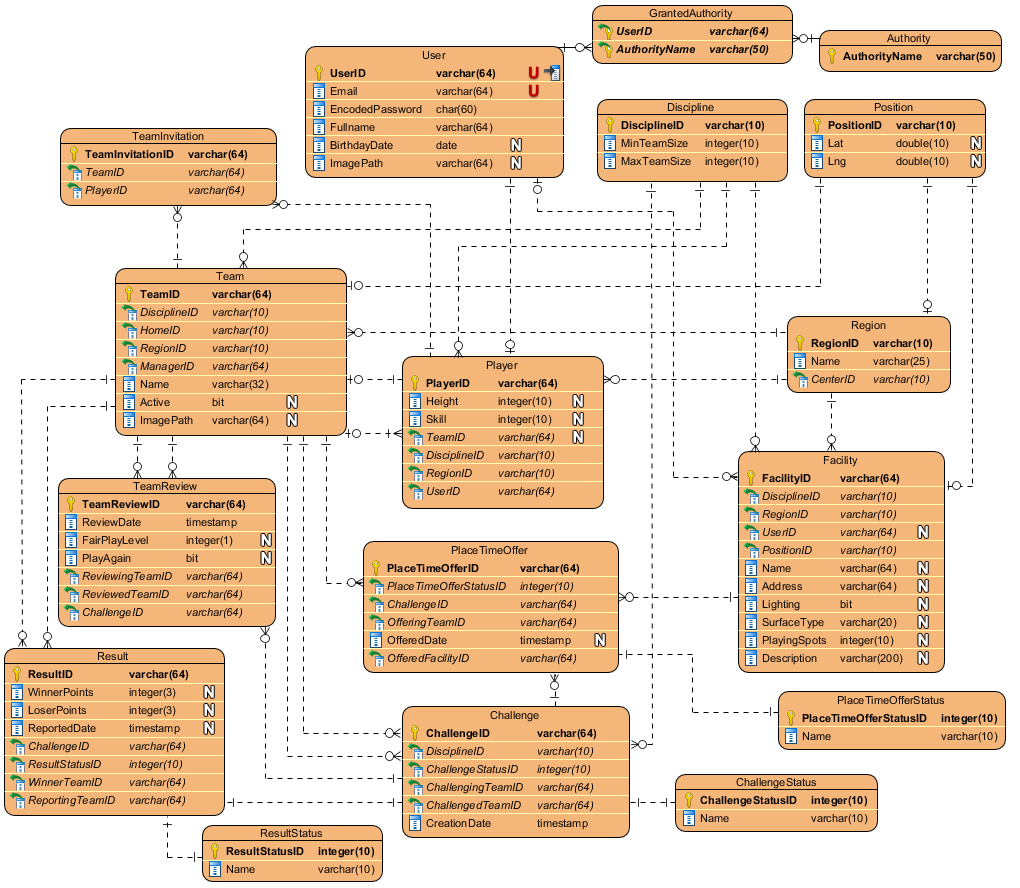
\includegraphics[width=1\linewidth]{04-projekt/rys/erd2.PNG}
\caption{Ogólny schemat metody rozwiązywania problemu optymalizacji wielokryterialnej}
\label{fig:diagram-trad-alg-opt}
\end{figure}

